%\documentstyle[epsf,twocolumn]{jarticle}       %LaTeX2e仕様
\documentclass[twocolumn]{jarticle}     %pLaTeX2e仕様(platex.exeの場合)
%\documentclass[twocolumn]{ujarticle}     %pLaTeX2e仕様(uplatex.exeの場合)
%%%%%%%%%%%%%%%%%%%%%%%%%%%%%%%%%%%%%%%%%%%%%%%%%%%%%%%%%%%%%%
%%
%%  基本バージョン
%%
%%%%%%%%%%%%%%%%%%%%%%%%%%%%%%%%%%%%%%%%%%%%%%%%%%%%%%%%%%%%%%%%
\setlength{\topmargin}{-45pt}
%\setlength{\oddsidemargin}{0cm} 
\setlength{\oddsidemargin}{-7.5mm}
%\setlength{\evensidemargin}{0cm} 
\setlength{\textheight}{24.1cm}
%setlength{\textheight}{25cm} 
\setlength{\textwidth}{17.4cm}
%\setlength{\textwidth}{172mm} 
\setlength{\columnsep}{11mm}

\kanjiskip=.07zw plus.5pt minus.5pt


% 【節が変わるごとに (1.1)(1.2) … (2.1)(2.2) と数式番号をつけるとき】
%\makeatletter
%\renewcommand{\theequation}{%
%\thesection.\arabic{equation}} %\@addtoreset{equation}{section}
%\makeatother

%\renewcommand{\arraystretch}{0.95} 行間の設定

%%%%%%%%%%%%%%%%%%%%%%%%%%%%%%%%%%%%%%%%%%%%%%%%%%%%%%%%
\usepackage[dvipdfmx]{graphicx}   %pLaTeX2e仕様(\documentstyle ->\documentclass)\documentclass[dvipdfmx]{graphicx}
\usepackage[dvipdfmx]{color}
\usepackage[subrefformat=parens]{subcaption}
\usepackage{colortbl}
\usepackage{multicol}
%%%%%%%%%%%%%%%%%%%%%%%%%%%%%%%%%%%%%%%%%%%%%%%%%%%%%%%%

\begin{document}

\twocolumn[
\noindent

\hspace{1em}
2020年10月23日
\hfill
\ \ 細川 岳大

\vspace{2mm}

\hrule

\begin{center}
{\Large \bf 進捗報告}
\end{center}
\hrule
\vspace{3mm}
]

% ‚ここから 文章 Start!

\section{今週やったこと}

\begin{itemize}
	%\item optuna
	\item FixmatchとGAを組み合わせた実験
\end{itemize}

\section{FixMatch + GA}
ラベルなし画像100枚取り出し,それらに対するラベルをGAによって探索する.
表\ref{tb:FTXpara},\ref{tb:GApara}に実験の設定を示す.
表\ref{tb:FTXpara}での精度をGAの目的関数とした.\\
 遺伝子は0から9の整数値をとる整数値コーディングとした.\\
 選択はサイズ2のトーナメント選択,交叉には二点交叉,突然変異は別の数値にランダムに移るように設定した.\\
 また,事前学習を表\ref{tb:FTXpre}の設定で行い,精度0.55(エラー率:0.45)であり,初期個体について,事前学習から予測したラベルに対し,各遺伝子座にエラー率の割合で突然変異させたものとした.
\begin{table}[h]
	\centering
	\caption{FixMatchの設定\label{tb:FTXpara}}
	\scalebox{1.0}{
		\begin{tabular}{|c|c|c|} \hline
			model&\multicolumn{2}{c|}{WideResNet16-2}\\ \hline\hline
			data set&\multicolumn{2}{c|}{cifar10}\\ \hline
			train &labeled&100\\ \cline{2-3}
			data&unlabeled&49650\\ \cline{2-3}
			&search&100\\ \hline
			batch size&labeled+search&64\\ \cline{2-3}
			&unlabeled&$64*7$\\ \hline
			val data&\multicolumn{2}{c|}{150}\\ \hline\hline
			num\_iterations&\multicolumn{2}{c|}{10000}\\ \hline
			optimizer&\multicolumn{2}{c|}{SGD(lr=0.1,momntum=0.9)}\\ \hline
			loss&\multicolumn{2}{c|}{cross\_entropy\_loss}\\ \hline
		\end{tabular}
	}
\end{table}

\begin{table}[h]
	\centering
	\caption{GAの設定\label{tb:GApara}}
	\scalebox{1.0}{
		\begin{tabular}{|c||c|} \hline
			個体数&5\\ \hline
			世代数&8\\ \hline
			交叉率&1.0\\ \hline
			突然変異率&0.06\\ \hline
		\end{tabular}
	}
\end{table}

\begin{table}[h]
	\centering
	\caption{事前学習の設定\label{tb:FTXpre}}
	\scalebox{1.0}{
		\begin{tabular}{|c|c|c|} \hline
			model&\multicolumn{2}{c|}{WideResNet16-2}\\ \hline\hline
			data set&\multicolumn{2}{c|}{cifar10}\\ \hline
			train &labeled&50\\ \cline{2-3}
			data&unlabeled&49750\\ \cline{2-3}
			batch size&labeled&64\\ \cline{2-3}
			&unlabeled&$64*7$\\ \hline
			val data&\multicolumn{2}{|c|}{200}\\ \hline\hline
			num\_iterations&\multicolumn{2}{c|}{10000}\\ \hline
			optimizer&\multicolumn{2}{c|}{SGD(lr=0.1,momntum=0.9)}\\ \hline
			loss&\multicolumn{2}{c|}{cross\_entropy\_loss}\\ \hline
		\end{tabular}
	}
\end{table}

\subsection{結果}
表\ref{tb:res},図\ref{fig}に結果を示す.
\begin{table}[h]
	\centering
	\caption{結果\label{tb:res}}
	\scalebox{1.0}{
		\begin{tabular}{|c||c|c|c|c|} \hline
			&\multicolumn{2}{c}{適応度}
			&\multicolumn{2}{|c|}{正答数}\\ \cline{2-5}
			&最大&平均&最大&平均\\ \hline\hline
			1世代&0.167&0.128&18&15.4\\ \hline
			2世代&0.167&0.120&17&15.8\\ \hline
			3世代&0.167&0.121&17&14.2\\ \hline
			4世代&0.167&0.124&17&13.8\\ \hline
			5世代&0.167&0.115&16&14.4\\ \hline
			6世代&0.180&0.131&16&13.6\\ \hline
			7世代&0.180&0.131&15&13.0\\ \hline
			8世代&0.180&0.136&14&12.6\\ \hline
		\end{tabular}
	}
\end{table}

\begin{figure}[h]
	\begin{center}
		\centering
		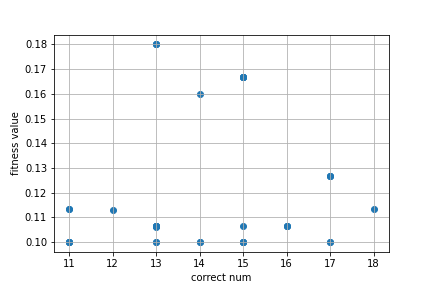
\includegraphics[scale=0.5]{img.png}
		\caption{散布図\label{fig}}
	\end{center}
\end{figure}

時間の都合上個体数,世代数共に低かったためあまり探索できていない.
また図\ref{fig}より,相関関係があまり成り立っていないことが分かる.
また,1個体の学習について1時間半ほど要した.

\subsection{考察}
出鱈目なラベルの割合が多いと精度との相関関係が薄くなる可能性があるので元のデータ数に対してsearchするデータ数の割合を小さくする必要がある.\\
一世代あたりの個体数が小さいために結果は悪い方向に収束していったと考えられる.あるいは,トーナメント選択で適応度の高いものが選ばれなかったことがあった.そのため適応度の低いものに制限をかけることも必要なのではないかと考えられる.\\
また選ばれたデータが悪いことを考えると,trainとvalのデータを世代ごとに入れ替えて,
交叉検証のような評価をする必要があるのではないかと思う.

\section{来週の課題}
\begin{itemize}
	\item 間違ったラベルの割合と精度の関係について調べパラメータの調整をする.
	\item cnnやrandomforestといった時間短縮につながる手法を組み込み実験を行う.
\end{itemize}

\end{document}


